\documentclass[Japanese]{dicomopapers}
%\documentclass[Japanese,noauthor]{dicomopapers}
\usepackage[dvips]{graphicx}
\usepackage{latexsym}

\def\Underline{\setbox0\hbox\bgroup\let\\\endUnderline}
\def\endUnderline{\vphantom{y}\egroup\smash{\underline{\box0}}\\}
\def\|{\verb|}

%概要投稿用余白調整ここから
\setlength{\Jauthorjreceivesep}{0.0mm}
\setlength{\Jreceivejabstsep}{0.0mm}
\setlength{\Jabstsepjkeyword}{0.0mm}
\setlength{\Jkeywordetitle}{0.0mm}
%概要投稿用余白調整ここまで

\begin{document}

% 和文表題
\title{SDNによる仮想デバイスを用いた\\セキュアなホームネットワークの検討}

% 英文表題
\etitle{A Study of SDN-based Security Platform for Home Networks}

% 所属ラベルの定義
\affiliate{DOSHISHA}{同志社大学大学院 理工学研究科\\Graduate School of Science and Engineering, Doshisha University}
\affiliate{MOBILITY}{同志社大学モビリティ研究センター\\Mobility Reserch Center, Doshisha University}

\author{塚崎 拓真}{TAKUMA TSUKASAKI}{DOSHISHA}
\author{滕 睿}{RUI TENG}{MOBILITY}
\author{佐藤 健哉}{KENYA SATO}{DOSHISHA}

% 表題などの出力
\maketitle

% 本文はここから始まる
\section{DICOMO概要テンプレートについて}
DICOMOでは,カメラレディの投稿論文について,\LaTeX 形
式の投稿フォーマットを提供しているが,論文発表申し込み
時の概要は2000字程度の文章を入力すること
としていた.しかしながら,従来の発表申し込み時の概要
はともすれば数行の短いものがあるなど,必ずしもクオリ
ティが保証されず,カメラレディ原稿に至らないケースも
散見された.

そこでDICOMOプログラム委員会では,概要のクオリティを
高めるため,論文投稿フォーマットを踏襲したA4判で1ページ
の概要テンプレートを提供し,これに基づいて発表申し込
み概要を登録していただくこととした.

この概要はあくまでアブストラクトであるため,細かい
章立ては不要である.しかし,図を挿入するなど,よりわ
かりやすく研究の位置づけや成果を示すことができる.本
概要テンプレートが著者の論文作成を助け,最終発表論文
のクオリティを向上させ,DICOMOの発展に役立つことを
期待している.

\begin{figure}[!tb]
  \centering
  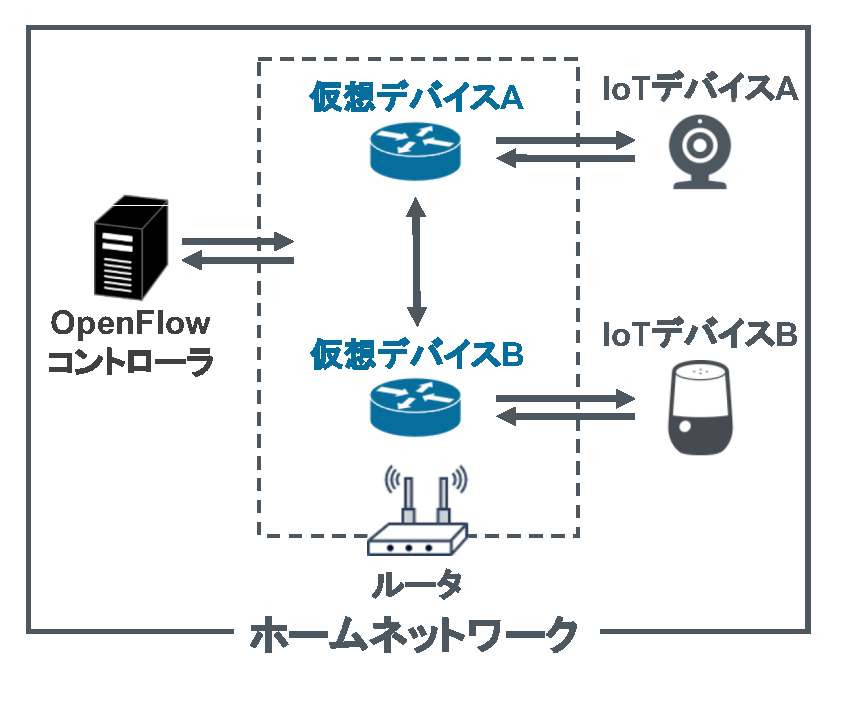
\includegraphics[width=\linewidth]{img/system.eps}
  \caption{提案手法の構成}
  \label{fig:syste}
\end{figure}

\section{概要作成に関する注意}
\begin{itemize}
  \item 概要のボリューム

        タイトル,著者,所属,概要を含めて本テンプレート1
        ページとする.

  \item 章立て

        章立ては無理に作らず,概要だけでよい.一方で,文章
        をわかりやすくする段落わけ・箇条書き等は推奨される.

  \item 図表の挿入

        成果をわかりやすく示す図表を挿入してもよい.

  \item 関連文献

        関連する文献を最後に記載してもよい.

  \item アブストラクト集(印刷物)との関係

        本概要はアブストラクト集には掲載されない.本概要をドラフトとして,
        別途提供される論文フォーマットによりあらためて論文を作成していただきたい.

  \item カメラレディ論文との書誌情報の整合

        本概要,および同時に登録する書誌情報(タイトル,著
        者名,所属,キーワード等)がプログラム編成・印刷に用いられる.
        誤りが生じないように,内容を明瞭に記述していただきたい.

\end{itemize}

\end{document}
